\chapter{Week3 :}

\section{Continuous Integration / Continuous Delivery \& Deployment}

\begin{defnbox}[title=CI/CD]
An \textbf{automated assembly line} for your software product: every change a developer
pushes travels through the same fixed sequence of steps (build, test, package, deploy)
without anyone having to run them by hand.
\end{defnbox}

\begin{keybox}[title={Three stages, three sets of goals}]
\begin{itemize}[leftmargin=1.5em, itemsep=3pt]
  \item \textbf{Continuous Integration} ---
        \begin{itemize}[leftmargin=1.5em, itemsep=1pt]
          \item merge code changes from multiple devs and ensure that they work together;
          \item catch bugs and integration problems as early as possible.
        \end{itemize}
  \item \textbf{Continuous Delivery} ---
        \begin{itemize}[leftmargin=1.5em, itemsep=1pt]
          \item constantly have the software in a ``deployable state'';
          \item automatically package the software, ready for deployment.
        \end{itemize}
  \item \textbf{Continuous Deployment} ---
        \begin{itemize}[leftmargin=1.5em, itemsep=1pt]
          \item automatically deploy to testing / staging / production.
        \end{itemize}
\end{itemize}
\tcblower
Each stage builds on the previous one: integration guarantees the merged code works,
delivery guarantees it can be shipped at any moment, and deployment actually ships it.
\end{keybox}

\subsection{The CI/CD Pipeline}

\begin{center}
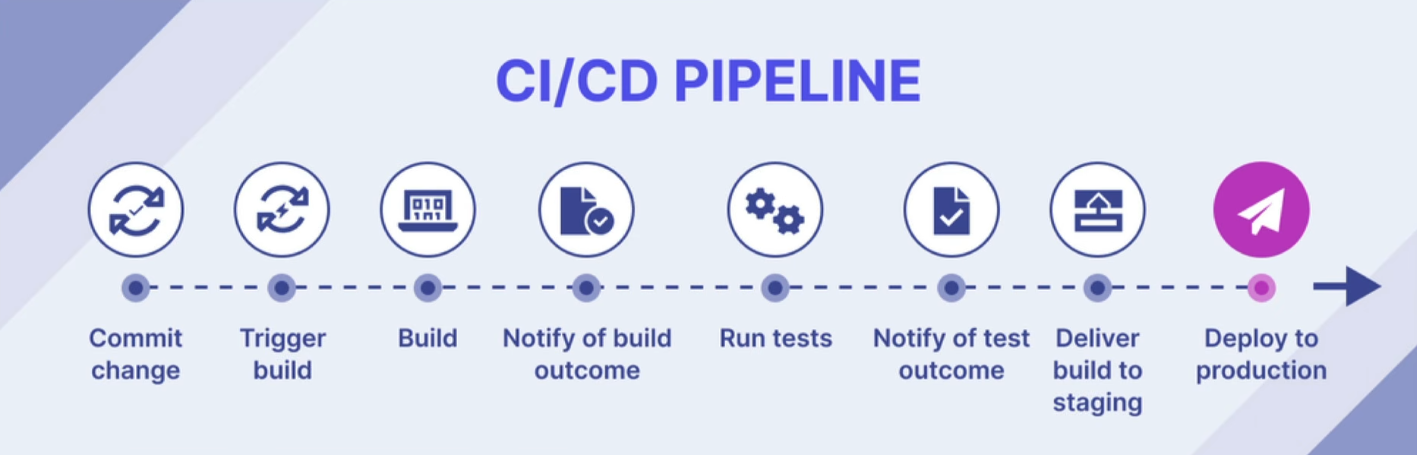
\includegraphics[width=\linewidth]{images/cicd-pipeline.png}
\end{center}

A single commit is enough to set the whole line in motion: the build is triggered
automatically, then the code is compiled and tested, and the team is \textbf{notified after
each stage}, so a failure is spotted minutes after the push. The first steps (commit
$\rightarrow$ test outcome) are \textbf{CI}. Delivering the build to staging is
\textbf{Continuous Delivery}. Pushing it to production automatically is
\textbf{Continuous Deployment}.

\begin{rembox}[title=Delivery vs.\ Deployment]
The difference is who presses the final button. With \textbf{Continuous Delivery}, every
change ends up as a release-ready package, but a human decides when to ship it. With
\textbf{Continuous Deployment}, that last step is automated too: any change that passes the
pipeline goes straight out to testing, staging or production.
\end{rembox}

\subsection{Our Pipeline for the Bootcamp}

\begin{center}
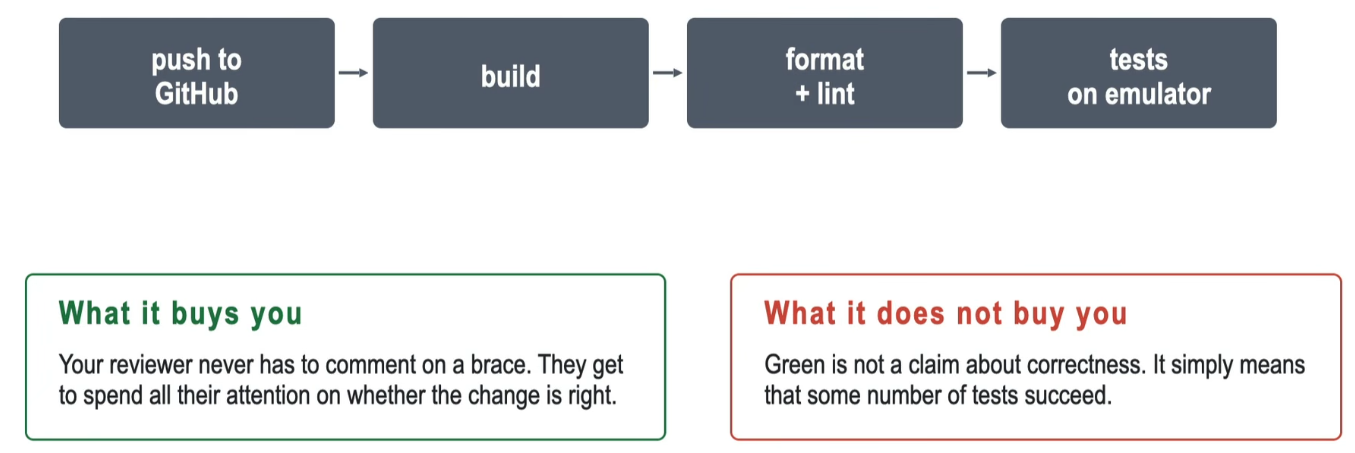
\includegraphics[width=\linewidth]{images/bootcamp-pipeline.png}
\end{center}

A concrete, smaller version of the pipeline above: every push to GitHub is built, then
automatically \textbf{formatted and linted}, then tested on an \textbf{Android emulator}.
It stops at CI (there is no delivery or deployment step). Because formatting and style are
checked by a machine, code review can focus on what matters. But a green check only says
that the tests we wrote pass; it can never be better than the test suite behind it.
